
The SparrowE wireless sensor nodes are custom designed for use in various research projects.
They are designed as a single PCB board which hosts all of the major components, such as: controller,
RF module, power supply and sensors. The main the main processing unit of the SparrowE nodes is an Atmega 
ZigBit 900MHZ RF module, which hosts both the microcontroller, an ATmega 1281V 8-bit microcontroller and the 
wireless transceiver, an AT86RF212 RF chip. These two components are connected via an SPI line inside the ZigBit 
module. The 8 bit, low power, Atmega 1281V microcontroller is connected to all of the node's sensors and its 
main function is to process the data received from them and pass it on to the RF transceiver. The AT86RF212 RF 
is a low power wireless transmission chip capable of sending signals to distances of up to a few kilometers, according 
to the official datasheet \cite{datasheetatmel}. It also provides an AES-128 compatible security module for data 
encryption and decryption.

\begin{figure}[ht] \centering
  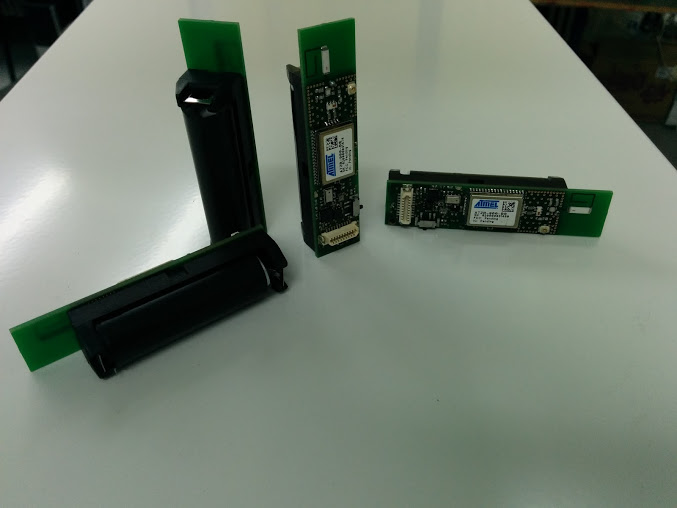
\includegraphics[width=0.45\textwidth]{img/sparrow-nodes.jpg}
  \caption{SparrowE wireless sensor nodes}
\end{figure}

In order to monitor its environment, the SparrowE wireless sensor node relies on 3 main sensor peripherals. The first is 
an Si7020 humidity and temperature sensor with incorporated ADC unit. The measurement resolution for relative humidity measurements
can vary between 8 and 12 bits, while the resolution for temperature measurements varies from 11 to 14 bits. The second sensor is 
an MPL3115A2 altimeter which can measure pressure and altitude. This sensor also has an incorporated ADC unit and can measure 
both altitude and pressure with a precision of up to 20 bits. The final sensor mounted on the SparrowE and the most important for 
earthquake and vibration monitoring is the LSM9DS0 IMU(Inertial Measurement Unit). This chip has 3 channels for linear acceleration measurement, 
3 channels for angular rate measurement and another 3 channels for magnetic field measurement. All data measurements are performed at a 
16 bit resolution. From this last sensor, the metric used by the presented application is the linear acceleration (measured in Gs).
All of the aforementioned sensors are connected to the microcontroller via a two-wire interface. Each of the has a different slave address so 
it is possible for the master, the Atmega 1281V controller, to communicate with all of them without interference from the others.

\begin{figure}[ht] \centering
  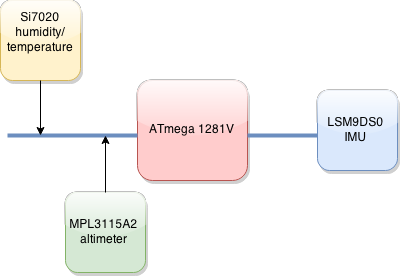
\includegraphics[width=0.5\textwidth]{img/i2c-connection.png}
  \caption{Sensors connected on two-wire interface}
\end{figure}

All the components on the SparrowE node function at a maximum supply voltage of 3.6V. The node can be powered in 2 ways: either from a lithium polymer battery 
cell or via an USB port. When powered via USB, a linear DC regulator is used to drop the supply voltage from the 5V of the USB line to the necessary 3.3V.

\subsection{Software}

The node software follows the same design ideea as the hardware one, so in order write code more easier, the node's firmware is a moddified arduino compatible one. This allows us to use existing libraries or to easily write our own.




